\documentclass{article}
\usepackage{hyperref}
\usepackage{graphicx}
\begin{document}
\title{}
\section{"The Cloud"}
\subsection{Definition}

\href{http://en.wikipedia.org/wiki/Cloud\_computing}{en.wikipedia.org—Cloud\_computing}
\subsubsection{Cloud computing is the use of computing resources (hardware and software) that are delivered as a service over a network (typically the Internet). The name comes from the use of a cloud-shaped symbol as an abstraction for the complex infrastructure it contains in system diagrams. Cloud computing entrusts remote services with a user's data, software and computation.}



\begin{figure}
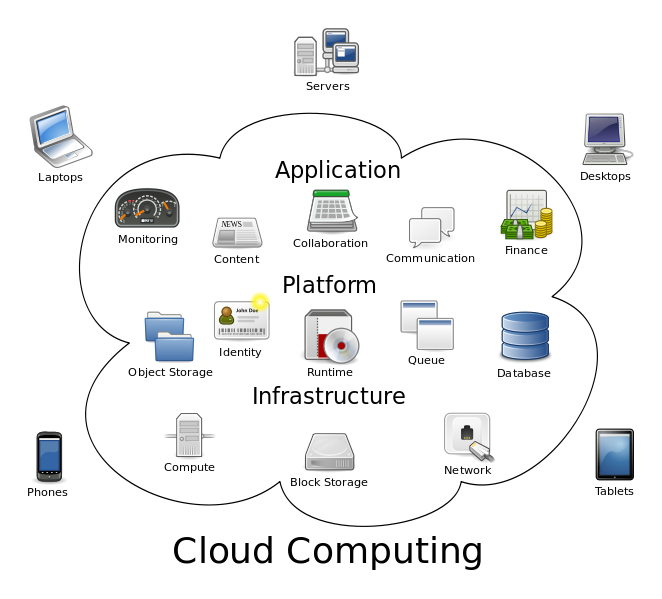
\includegraphics{Cloud_computing.png}
\caption{Cloud\_computing}
\label{fig:att1}
\end{figure}
\subsection{Types}

\href{http://theinstitute.ieee.org/technology-focus/technology-topic/a-view-inside-the-cloud}{theinstitute.ieee.org—a-view-inside-the-cloud}
Software as a Service (SaaS) [GMail, Hotmail, Salesforce]

With SaaS, cloud providers install and operate application software such as 
\href{http://www.salesforce.com/}{Salesforce}, an online sales management tool that users can access.
“You have the least flexibility with SaaS, because you are just using the provider’s software, but you get dramatically better economies of scale,” Pasik says. Users don’t have to worry about managing the infrastructure or platform on which the application runs—the cloud provider handles that.

High 'Economies of Scale'  benefits.  Few and highly controlled set of features.  Benefits derived from many people using that same tool.
Platform as a Service (PaaS) [Google Apps, Office 365]

PaaS includes all the features of IaaS, but clients use the provider’s computing platform, which typically includes an operating system, developer tools, database, and Web server. Users can develop and run their software in the cloud without the cost and complexity of buying and managing the underlying hardware.

Medium 'Economies of Scale' benefits.  Controlled set of tools but freedom is given to leverage the platform in different ways.  Benefits derived from many people using similar toolsets.
Infrastructure as a Service (IaaS) [AWS, Rackspace]

With IaaS, clients have access to virtual servers in the service provider’s data center.

Lower 'Economies of Scale' benefits… but greater then running your own hardware.
\subsection{Deployment Models}
Public Cloud

Community Cloud

Hybrid Cloud

Private Cloud

\section{Why?}
Value Generation (Impact++) vs. Cost

By increasing the number of customers and improving specialization, the cost of production (of services) can be driven down. Economies of scale kicks in. When some one else could provide the service for less, do we consider the Opportunity cost of maintaining the status quo?  What 'higher value' things could we be doing to make the organization more productive?
\subsection{Enter Wentworth Research Program}
Source: George Cox, Time to Reshape the IS Department? Wentworth Research Program (now part of Gartner EXP, Stamford, CT), June 1994.



\begin{figure}
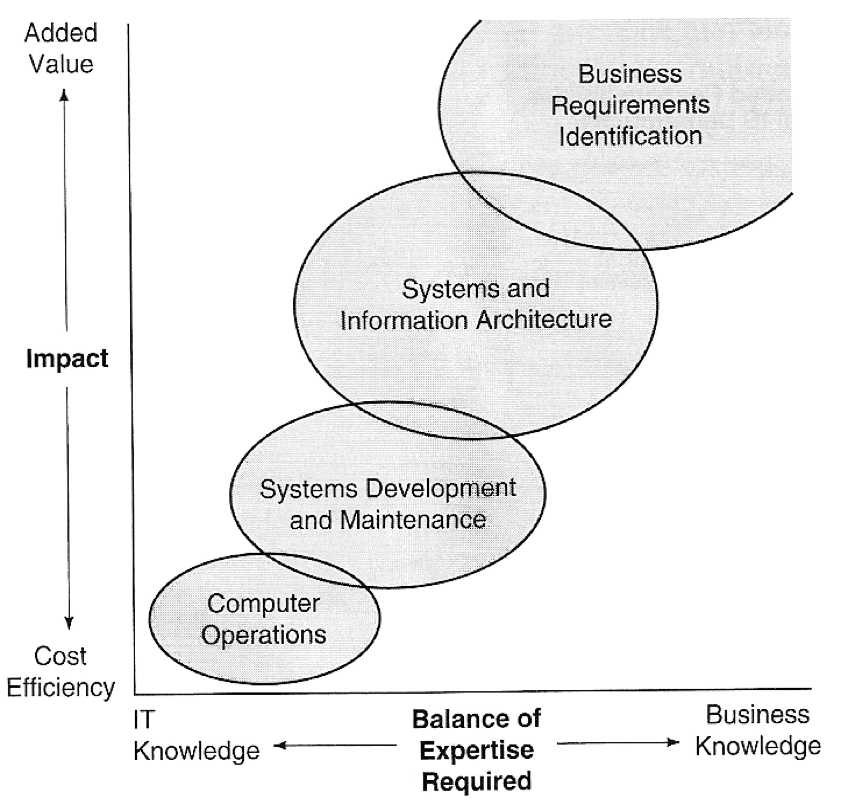
\includegraphics{time-to-reshape-it.png}
\caption{time-to-reshape-it}
\label{fig:att2}
\end{figure}
As IT professionals, we can have a disproportionate impact on the good of the organization if we develop expertise that helps our users and co-workers get their work done.

\section{What is a Service?}
\subsection{Basic}
Inputs + Functionality = Output

\subsection{Formal}
See: Journal of Software, July 2006 > 

\subsection{Practical}
Inputs = (effort, data, contract, connection)

Functionality (unknown to user)

Output = (results)

\subsection{Representation}



\begin{figure}
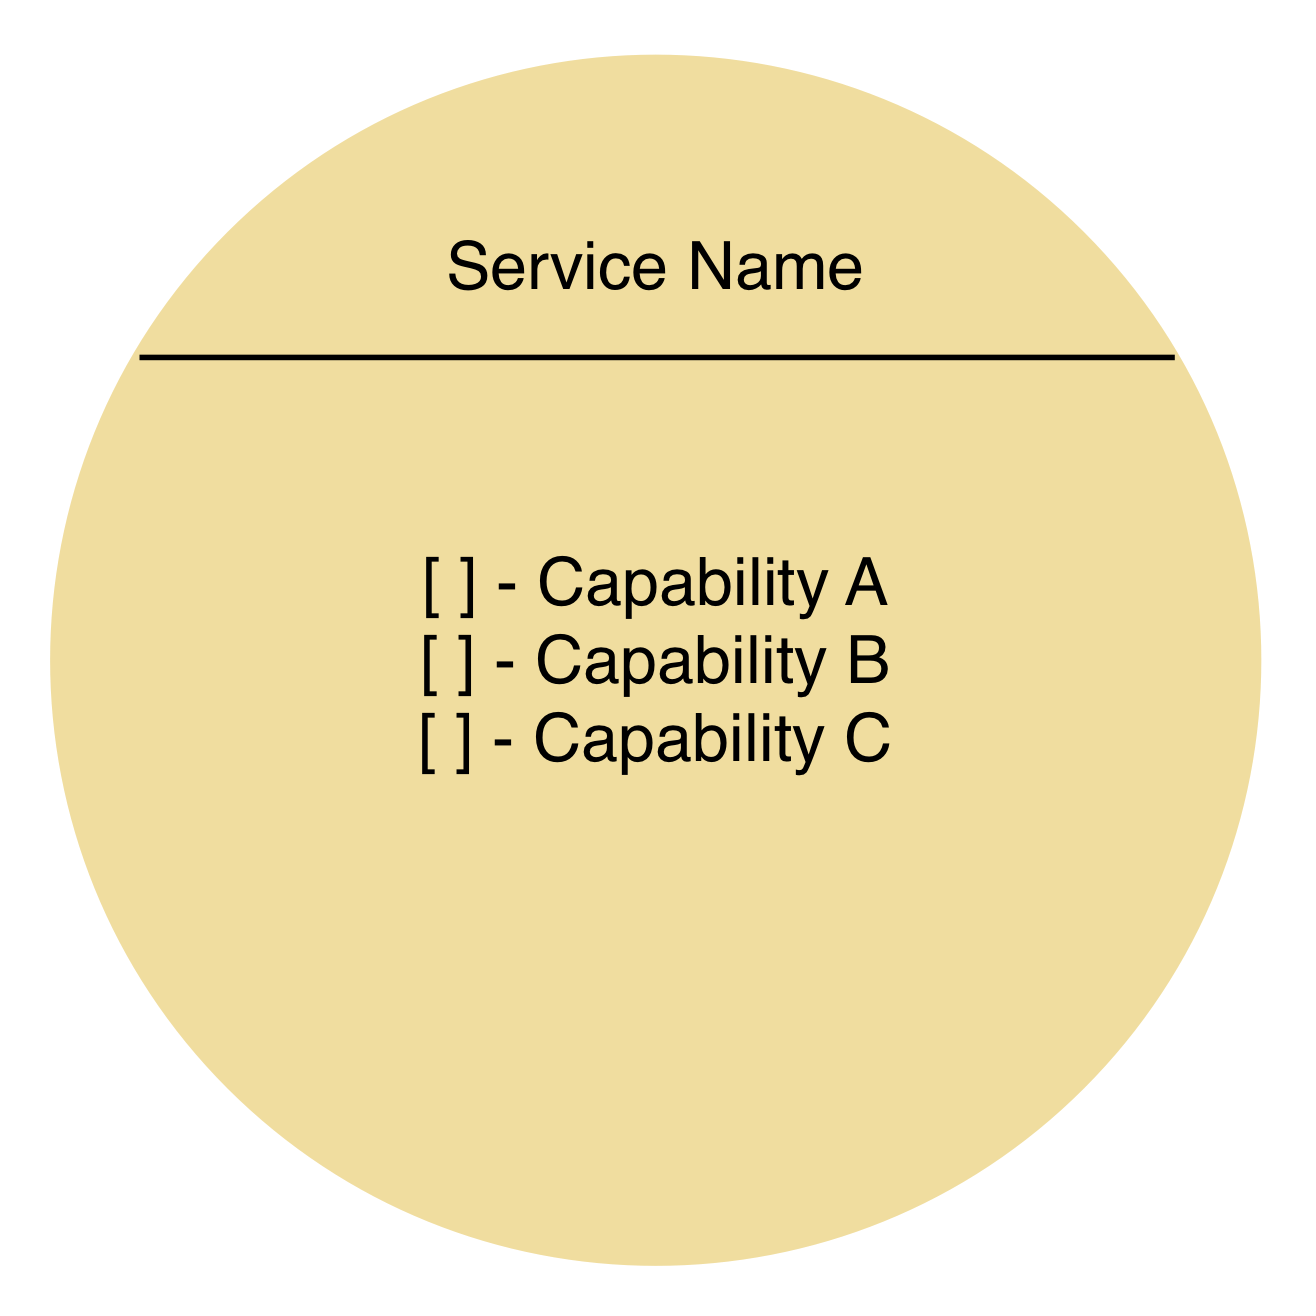
\includegraphics{Chorded-Circle.png}
\caption{Chorded-Circle}
\label{fig:att0}
\end{figure}
\section{Building the Services Oriented Enterprise (SOE)}
\subsection{Service Management}
\subsubsection{Information Technology Infrastructure Library (ITIL)}
Definitions pulled from: 
\href{http://en.wikipedia.org/wiki/Information\_Technology\_Infrastructure\_Library}{en.wikipedia.org—Information\_Technology\_Infrastructure\_Library}
Service Strategy

provides guidance on clarification and prioritization of service-provider investments in services
Service Design

provides good-practice guidance on the design of IT services, processes, and other aspects of the service management effort
Service Transition

relates to the delivery of services required by a business into live/operational use, and often encompasses the "project" side of IT rather than "BAU" (
\href{http://en.wiktionary.org/wiki/business\_as\_usual}{business as usual})
Service Operation

Continual Service Improvement

\subsection{Enterprise Architecture}
\subsubsection{Definitions}
Gartner:  


\href{http://www.gartner.com/it-glossary/enterprise-architecture-ea/}{www.gartner.com—enterprise-architecture-ea}Human readable: 

\subsubsection{Zachman Framework for Enterprise Architecture}
Columns:

"What"

Rows

"Scope"

\subsection{Service-oriented Architecture}

\href{http://en.wikipedia.org/wiki/Service-oriented\_architecture}{en.wikipedia.org—Service-oriented\_architecture}
 "


\href{http://en.wikipedia.org/wiki/Software\_engineering}{software engineering}
\href{http://en.wikipedia.org/wiki/Methodologies}{methodologies}
\href{http://en.wikipedia.org/wiki/Software}{software}
\href{http://en.wikipedia.org/wiki/Interoperability}{interoperable}
\href{http://en.wikipedia.org/wiki/Service\_\%28systems\_architecture\%29}{services}
\href{http://en.wikipedia.org/wiki/Function\_\%28computer\_science\%29}{functionalities}
\href{http://en.wikipedia.org/wiki/Software\_component}{software components}
\href{http://en.wikipedia.org/wiki/Modular\_programming}{pieces of code}
\href{http://en.wikipedia.org/wiki/Data\_structure}{data structures}
\href{http://en.wikipedia.org/wiki/Code\_reuse}{reused}
\href{http://en.wikipedia.org/wiki/Systems\_design}{design}
\href{http://en.wikipedia.org/wiki/Systems\_development}{systems development}
\href{http://en.wikipedia.org/wiki/Systems\_integration}{integration}\subsubsection{Principles}
Basics

loosely couple at all costs. services do not require a particular operating system or technology.  services should remain unassociated until runtime and there should be no embedded links between systems

all communications must be formalized and take place on documented channels through documented interfaces

in order to build new services on top of other services that can offer any sort of 'contract' about performance, you need 'underpinning' contracts.  Service-level Agreements (SLAs) are part of ITIL (Service Management).

Erl View

	•	
\href{http://en.wikipedia.org/wiki/Service-oriented\_architecture#Service\_contract}{Standardized service contract}: Services adhere to a communications agreement, as defined collectively by one or more service-description documents.
	•	
\href{http://en.wikipedia.org/wiki/Service\_loose\_coupling}{Service loose coupling}: Services maintain a relationship that minimizes dependencies and only requires that they maintain an awareness of each other.
	•	
\href{http://en.wikipedia.org/wiki/Service\_abstraction}{Service abstraction}: Beyond descriptions in the service contract, services hide logic from the outside world.
	•	
\href{http://en.wikipedia.org/wiki/Service\_Reusability\_Principle}{Service reusability}: Logic is divided into services with the intention of promoting reuse.
	•	
\href{http://en.wikipedia.org/wiki/Service\_Autonomy\_Principle}{Service autonomy}: Services have control over the logic they encapsulate.
	•	
\href{http://en.wikipedia.org/wiki/Service\_Statelessness\_Principle}{Service statelessness}: Services minimize resource consumption by deferring the management of state information when necessary
	•	
\href{http://en.wikipedia.org/wiki/Service\_discovery}{Service discoverability}: Services are supplemented with communicative meta data by which they can be effectively discovered and interpreted.
	•	
\href{http://en.wikipedia.org/wiki/Service\_Composability\_Principle}{Service composability}: Services are effective composition participants, regardless of the size and complexity of the composition.
Some authors also include the following principles:
	•	
\href{http://en.wikipedia.org/wiki/Service\_Granularity\_Principle}{Service granularity}: A design consideration to provide optimal scope and right granular level of the business functionality in a service operation.
	•	Service normalization: Services are decomposed and/or consolidated to a level of normal form to minimize redundancy. In some cases, services are denormalized for specific purposes, such as performance optimization, access, and aggregation.
\href{http://en.wikipedia.org/wiki/Service-oriented\_architecture#cite\_note-9}{[9]}
	•	Service optimization: All else equal, high-quality services are generally preferable to low-quality ones.
	•	Service relevance: Functionality is presented at a granularity recognized by the user as a meaningful service.
	•	Service 
\href{http://en.wikipedia.org/wiki/Encapsulation\_\%28computer\_science\%29}{encapsulation}: Many services are consolidated for use under the SOA. Often such services were not planned to be under SOA.
	•	Service location transparency: This refers to the ability of a service consumer to invoke a service regardless of its actual location in the network. This also recognizes the discoverability property (one of the core principle of SOA) and the right of a consumer to access the service. Often, the idea of service virtualization also relates to location transparency. This is where the consumer simply calls a logical service while a suitable SOA-enabling runtime infrastructure component, commonly a service bus, maps this logical service call to a physical service.

\subsubsection{Why all this work? Agility => Alignment => Productivity++ !  Lego building blocks can be assembled and rearranged.  The closer the Service's functionality is to the requirements of the business, the more productive the business will be.}
Case: Amazon vs. Google > Steve Yegge's "Stevey's Google Platforms Rant"

Engineer at Google released a rant on Google+ around Oct 2011.

He had worked at Amazon for 6.5 years and, when written, had worked at Google for about the same.

Realization… Amazon in 2002 has a major period each year where they experience a massive jump in traffic (Holidays).

Discussing Jeff Benzos (founder + CEO of Amazon).  In 2002 Jeff issued a mandate:

1) All teams will henceforth expose their data and functionality through service interfaces.

2) Teams must communicate with each other through these interfaces.

3) There will be no other form of interprocess communication allowed: no direct linking, no direct reads of another team's data store, no shared-memory model, no back-doors whatsoever. The only communication allowed is via service interface calls over the network.

4) It doesn't matter what technology they use. HTTP, Corba, Pubsub, custom protocols -- doesn't matter. Bezos doesn't care.

5) All service interfaces, without exception, must be designed from the ground up to be externalizable. That is to say, the team must plan and design to be able to expose the interface to developers in the outside world. No exceptions.
Lessons from a massive undertaking of building SOA at Amazon:

pager escalation can get hard.  need metrics and reporting

every single one of your peer teams becomes a potential denial of service

monitoring and QA are the same thing in SOAs

a universal service registration mechanism is a powerful thing to have

follow on benefits are compelling

This leads Steve Yegge to explain that, as painful as the transition to SOA was, it was the Right Thing to do.  Steve goes on to stress that Amazon's abilities as a provider of Infrastructure and a Platform far outstrip Google's because of one ULTIMATE THING:

Accessibility!  Not like WCAG Accessibility… like basic fundamental access to information + functionality.  If someone cannot access something they should be able to it represents a huge roadblock to an Organization's success.

Morale of the story:  There is evidence that an organization is able to thrive in their market and easily develop marketable value-add functionality (seemingly) due to their adoption of SOA.  They accomplished this by using 'Services' as Lego blocks and combing their blocks in a wide variety of ways.

\subsection{Choreography of Services}
\subsubsection{Know your Service Offerings!}
Top-Down (Design) Approach

Think about what a service represents, what it needs for input, what it needs in terms of a contract.  Define them!
Define Service from from the Strategic Level => Tactical Level => Operational Level (Implementation).

Bottom-UP (Organic/Discovery/Cataloguing) Approach

Examine the environment.  Find all the systems and services currently available in the organization.  Document their contracts and required inputs.
Define Service from an existing Implementation (Operational Level) => Tactical Level => Strategic Level

\subsubsection{Like Tri-color toothpaste, Services have Layers.  Keep them separate until use.}
Enterprise Service Layer - The University-wide view of a particular Service.  What does it do from the "normal" user's perspective?

Domain Service Layer - The domain expert's (Business) view of a particular Service.  What does this do as part of a particular business process?

Application Service Layer - The technologist's (IT) view of a particular Service.  How does it do what it is supposed to do?

Governance
\end{document}
